\chapter{Fundamento teórico}\label{chap:teoria}
En este capítulo se presentan los conceptos y términos fundamentales que se utilizan en el
proyecto, para proporcionar una base teórica sobre la que se desarrolla el trabajo. Se discuten
los conceptos de \textit{data lake}, \textit{procesos ETL} y \textit{dashboards}, que son
fundamentales para el desarrollo del proyecto.

\section{Paradigmas de almacenamiento de datos}\label{sec:paradigmas}


\subsection{Data lake}\label{sec:datalake}
Los \textit{data lakes}\footnote{\url{https://aws.amazon.com/es/what-is/data-lake/}}
son almacenes de datos que guardan grandes cantidades de datos de manera no
estructurada~\cite{mier2023dashboards}. En el ámbito de una empresa, un \textit{data lake}
contiene datos de diferentes fuentes de valor no considerado hasta su análisis, de manera
que su explotación posterior y su análisis no depende de una estructuración y transformación
compleja, reduciendo los costes de los procesos ETL derivados, una flujo de tareas que se
aplican sobre la información para ingestarla.. Esto
no quiere decir que no se apliquen estos procesos a los datos, sino que se aplican de manera
más flexible y básica que en otras estructuras de almacenamiento de datos con esquemas
predefinidos, como los \textit{data warehouses}.~\cite{pwint2018data}

A diferencia de los \textit{data warehouses}, los \textit{data lakes} no tienen un
esquema definido, lo que permite almacenar datos \textit{heterogéneos}. Esto permite
almacenar grandes cantidades de información sin tener que definir un esquema de antemano,
lo que puede ser útil en aquellos casos en los que no se conoce la estructura de los
datos que se van a almacenar.

Estas características de los \textit{data lakes} hacen que sean más atractivos en el sector
empresarial de cara al análisis de información, en contraste con las estructuras planteadas
normalmente en el campo de la investigación académica.

Para consultar esta gran cantidad de datos almacenados, se suelen utilizar técnicas de
visualización de datos, como los \textit{dashboards}, herramientas de visualización que
permiten observar los datos de manera sencilla y eficiente.

\newpage{}
\section{Procesos ETL}\label{sec:etl}
Los procesos ETL~\cite{mier2023dashboards} son procesos que combinan datos de múltiples
fuentes en un único destino, transformando los datos en un formato común. Estos procesos
se utilizan para extraer datos de diferentes fuentes, transformarlos en un formato común
y cargarlos en un destino común, como puede ser un \textit{data lake}.

% \subsection{Características}
Los procesos ETL, fundamentales en el ámbito de la gestión de datos, presentan atributos
distintivos que facilitan la integración eficaz de información procedente de diversas fuentes:

\begin{itemize}
	\item \textbf{Adaptabilidad:} los procesos ETL deben de adaptarse a la estructura de los
		datos de la fuente de origen, ya que dichas fuentes pueden tener diferentes estructuras
		y tener tipos de datos diferentes (la característica de \textit{heterogeneidad} de los
		datos que ya se ha mencionado).
	\item \textbf{Escalabilidad:} otra de las características clave de los procesos ETL es que sean
		escalables, ya que los datos que se muestran en los dashboards suelen ser datos que se generan
		de manera continua, y por lo tanto los procesos ETL deben ser capaces de procesar grandes
		cantidades de datos de manera eficiente. En ocasiones, los procesos ETL se pueden realizar en
		\textit{streaming}, lo que significa que los datos se procesan en tiempo real a medida que se
		generan.
\end{itemize}

\newpage{}
\subsection{Funcionamiento}
Los procesos ETL se dividen en tres fases principales: \textit{extracción}, \textit{transformación}
y \textit{carga}, como se muestra en el sigiuente diagrama:

\begin{minipage}{\linewidth}
	\centering
	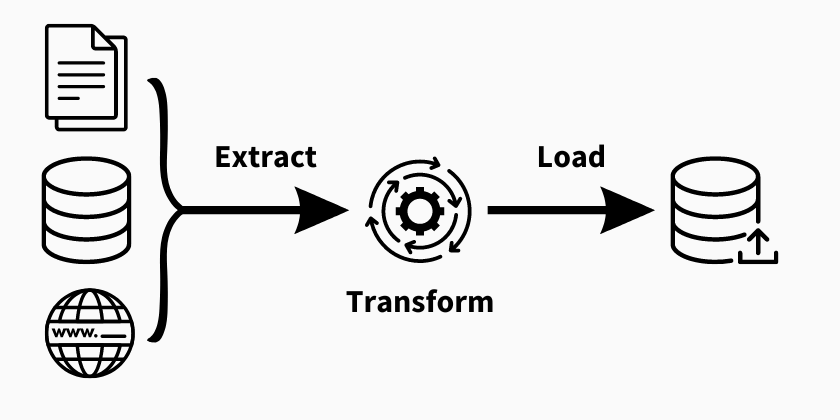
\includegraphics[width=0.8\textwidth]{etl.png}
	\captionof{figure}{Fases de un proceso ETL (trabajo propio)}
\end{minipage}

Al comienzo del proceso, se tienen datos presúntamente heterogéneos que no se pueden analizar de
manera eficiente. Tras aplicar todos los pasos de las fases anteriores, se obtiene un conjunto de
datos homogéneos y listos para ser analizados en el destino indicado (en el caso de este proyecto,
un \emph{data lake}).

\paragraph{Extracción (1)}
En este proceso se extraen los datos de las fuentes de datos, que pueden ser bases de datos, logs,
APIs, etc. En este paso, se pueden aplicar filtros para extraer solo los datos que se necesiten, y
se pueden extraer datos de múltiples fuentes \emph{heterogéneas}.

En algunos casos, los datos se pueden extraer de manera incremental, es decir, solo se extraen los
datos que han cambiado desde la última extracción. Esto puede ser útil para reducir el tiempo de
procesamiento y el volumen de datos que se almacenan.

En otros casos, los datos se pueden extraer de manera continua, es decir, se extraen los datos en
tiempo real según se van generando. Esto puede ser útil para procesar datos que se generan en tiempo
real, como logs o datos de sensores.

\newpage{}
\paragraph{Transformación (2)}
En este proceso se transforman los datos extraídos en la fase anterior, normalmente aplicándoles
un proceso de limpieza y transformación a un formato común. En este paso, se pueden aplicar
diferentes operaciones a los datos, como la limpieza, la agregación, la normalización, la conversión
de formatos, etc.

Una transformación especialmente importante que se suele reaizar durante este proceso es la limpieza,
revisión y corrección de los datos extraídos, para asegurar que se almacena información correcta y
consistentes. Durante esta fase se contemplan operaciones más complejas, como pueden ser la agregación
de datos, la conversión de formatos, la normalización de datos, el cifrado, etc.

Estos procesos de transformación son vitales cuando el sistema maneja una gran cantidad de datos heterogéneos
de múltiples fuentes de manera simultánea, como puede ser el caso de un \textit{data lake} o un \textit{data
warehouse}. En el caso del primero, no es necesaria la transformación de los datos a un formato común, pero si
otros procesos clave como la limpieza y la normalización de los datos, entre otros.

\paragraph{Carga (3)}
En este proceso se cargan los datos transformados en el destino final. Frecuentemente, los datos se
almacenan en una data warehouse o data lake para su posterior análisis.

La frecuencia del proceso de carga depende de la naturaleza de los datos y de las necesidades del
negocio, como ya se ha descrito en el proceso de extracción.

Tras completar este proceso, los datos están listos para ser analizados y visualizados desde las arquitecturas
de datos que almacenen la información.

\newpage{}
\subsection{Alternativas}
Aunque lo más común es el flujo anteriormente explicado de \textit{extracción}, \textit{transformación} y
\textit{carga}, existen algunos flujos y procesos alternativos que evitan algunos de estos pasos, normalmente
en casos específicos que se beneficien del cambio:

\begin{itemize}
	\item \textbf{Virtualización de datos:} capa virtual de abstracción que permite acceder a los datos de las
		fuentes sin necesidad de extraerlos. Esto permite ahorrar espacio de almacenamiento y tiempo de procesamiento,
		pero suele ser menos eficiente en términos de rendimiento y no es compatible con todas las arquitecturas de
		datos.

		\begin{minipage}{\linewidth}
			\centering
			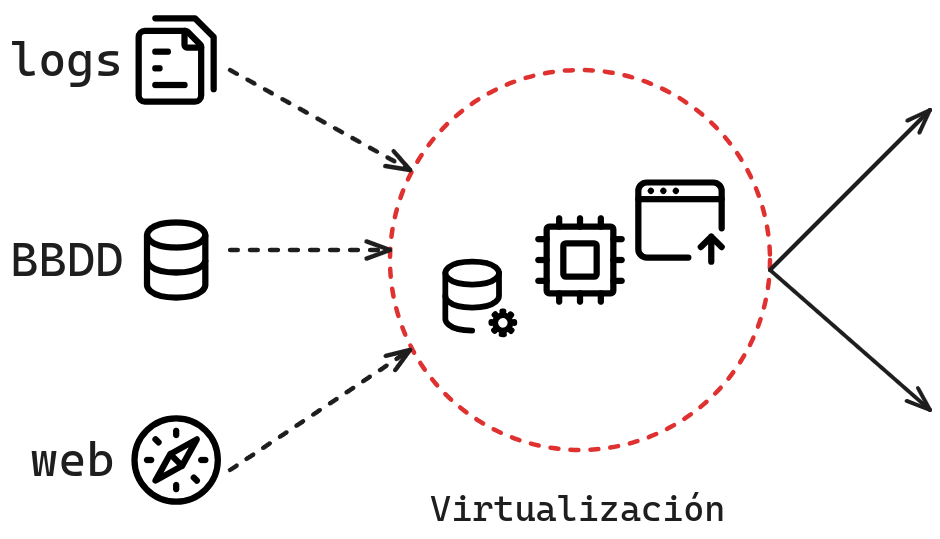
\includegraphics[width=0.65\textwidth]{virt.png}
			\captionof{figure}{Ejemplo de flujo con virtualización (trabajo propio)}
		\end{minipage}
	\item \textbf{Proceso \textit{ELT}\footnote{\url{https://www.ibm.com/topics/elt}}:} en lugar de transformar
		los datos antes de cargarlos en el destino, se cargan los datos en bruto y se transforman en el destino.
		Funciona bien para grandes conjuntos de datos sin estructura que requieran una carga (o recarga) contínua,
		aunque, al igual que la virtualización, puede ser menos eficiente o incompatible con algunas arquitecturas
		de datos, como los \textit{data warehouses}.

		\begin{minipage}{\linewidth}
			\centering
			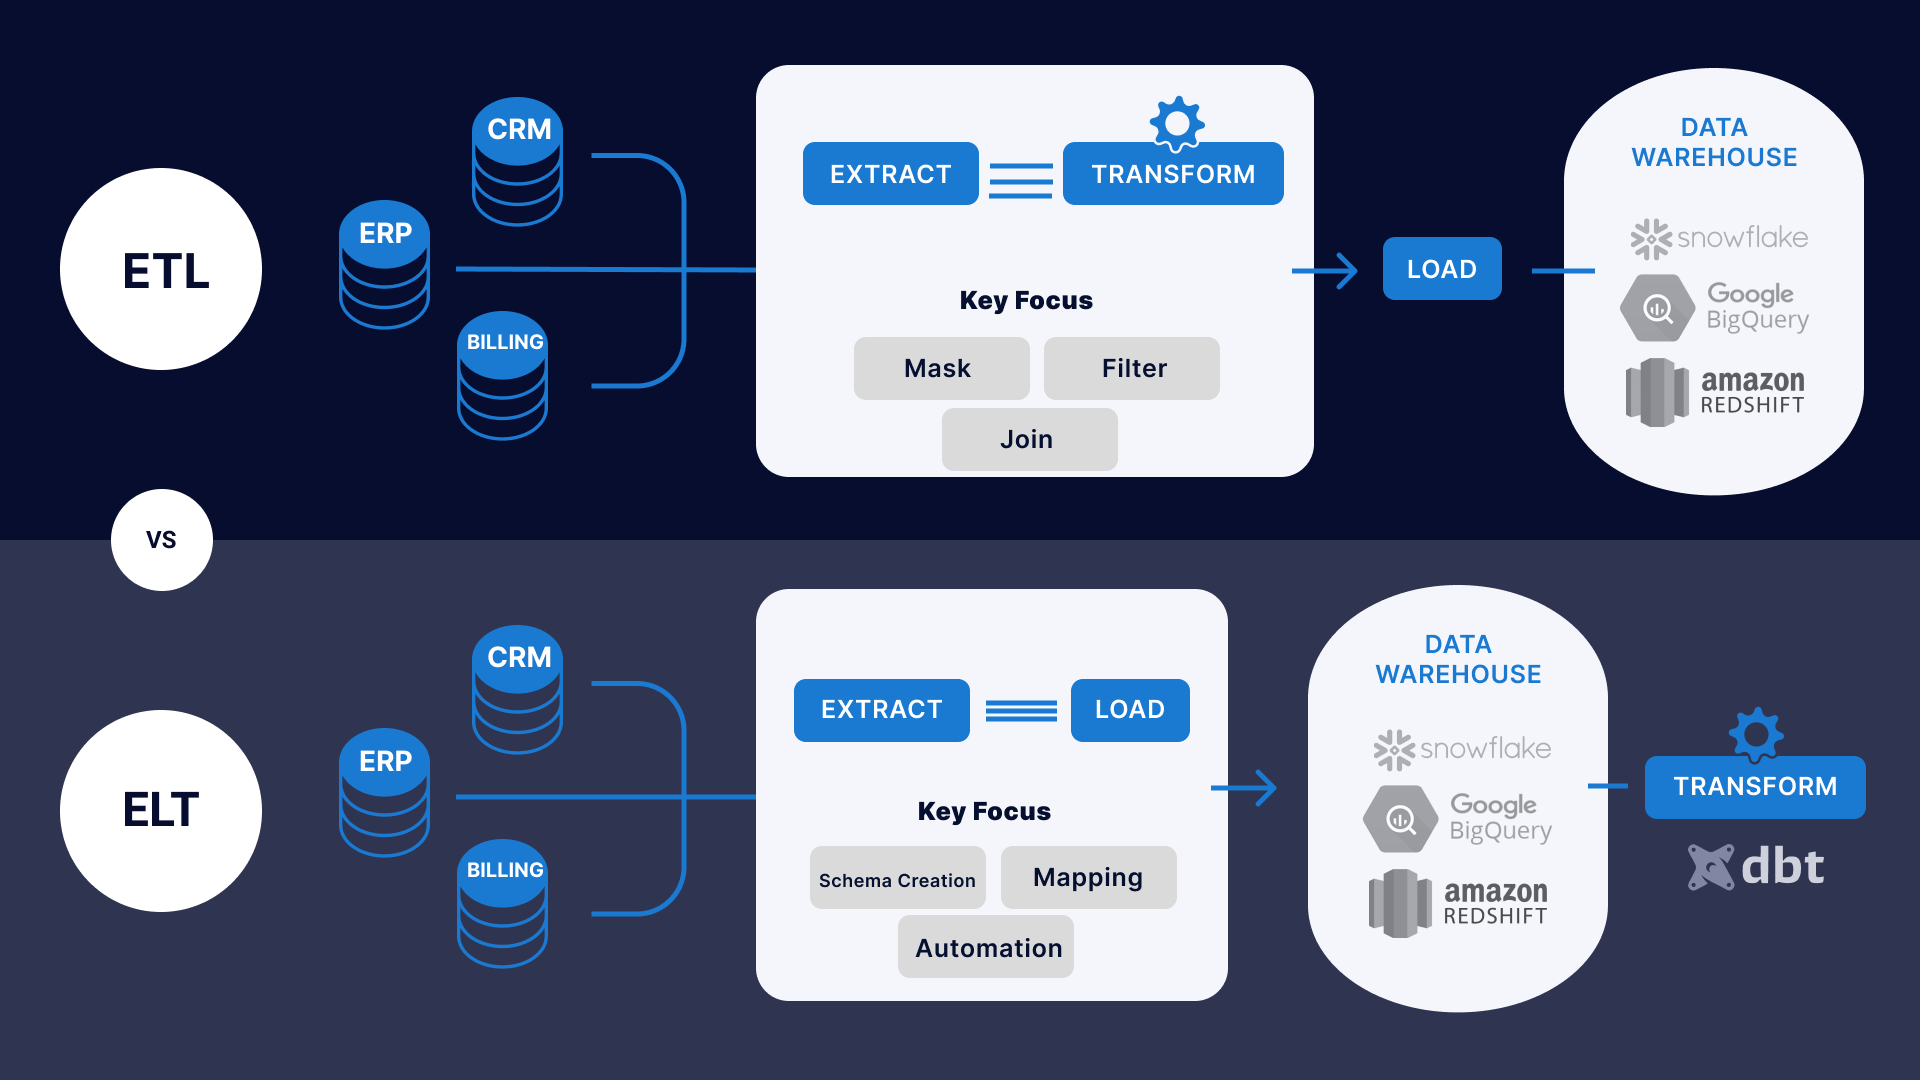
\includegraphics[width=0.75\textwidth]{elt.png}
			\captionof{figure}{Diagrama de flujo de un proceso \textit{ELT} (trabajo propio)}
		\end{minipage}
\end{itemize}


\newpage{}
\section{Dashboards}\label{sec:dashboards}
\paragraph{Definición}
La palabra \textit{dashboard}, que traducido de manera literal significa \textit{cuadro de mandos},
es un término que se utiliza para referirse a cualquier interfaz gráfica que muestre información
relevante de manera visual sobre un proceso o negocio. Aunque el término se utiliza en
muchos ámbitos: indicadores comerciales, de producción, de marketing, de calidad, de recursos
humanos\ldots, en este proyecto se utilizará en el ámbito de la monitorización de sistemas y
procesos de negocio.

En el ámbito de deste proyecto, los dashboards reflejan en tiempo real el rendimiento de
actividades o procesos de negocio, y se utilizan para tomar decisiones informadas sobre los
mismos. En el caso de una empresa, un dashboard puede mostrar desde el rendimiento de la
plataforma en tiempo real hasta un reflejo del de las ventas, y permitir a los directivos tomar
decisiones informadas sobre el futuro de la empresa.

\paragraph{Características}
Los dashboards cuentan con una serie de características que los hacen útiles para la toma de
decisiones:~\cite{mier2023dashboards}

\begin{itemize}
	\item \textbf{Visualización de datos:} es la característica fundamental de cualquier
		cuadro de mandos, y aquella que determina su utilidad. La visualización de datos
		es la ciencia de presentar los datos de manera que se pueda extraer información útil
		y realizar decisiones informadas sobre ellos. Un buen dashboard cuenta con gráficas,
		tablas, indicadores, etc. que permiten al usuario entender la información que se
		está presentando con un conocimiento técnico mínimo.
	\item \textbf{Interactividad y personalización:} un dashboard debe permitir al usuario
		interactuar con los datos (filtrarlos, ordenarlos, profundizar en ellos...) y ajustar
		la información que se muestra a cada proceso o negocio que se esté evaluando.
		Esta capacidad asegura que el dashboard se adapte tanto a las necesidades actuales
		como a las evoluciones futuras de lo que se esté analizando.
	\item \textbf{Accesibilidad y portabilidad:} un dashboard debe ser accesible desde una
		variedad de situaciones y dispositivos, manteniendo su funcionalidad y forma. Aunque
		normalmente los dashboards se analizan en pantallas grandes, es importante que también
		se puedan consultar en otras circunstancias, como dispositivos móviles.
\end{itemize}

\newpage{}
\subsection{Dashboards planteados}
Para el sistema que se describe, se plantean dos tipos de dashboards diferentes:

\begin{itemize}
	\item \textbf{Dashboards internos}: que reflejan el rendimiento de la plataforma en tiempo real.
	\item \textbf{Dashboards externos}: que reflejan el rendimiento de las ventas y permiten a los
	      clientes tomar decisiones informadas sobre su negocio.
\end{itemize}

Hay que destacar que los dashboards externos son diferentes a los dashboards de monitorización, tanto
en el contenido que presentan como en la manera de acceder a ellos: mientras que los dashboards de
monitorización serán de uso interno exclusivo, los dashboards externos deben estar disponibles para
los clientes de las empresas que los contraten.

% mover esta sección a la valoración de alternativas cuando se tenga
% \section{Componentes del sistema}\label{sec:componentes}
% En el \textit{stack} tecnológico escogido para el proyecto se manejan
% diferentes términos y conceptos que son necesarios desarrollar para
% entender el funcionamiento del sistema.

% \subsection{Tópico}\label{subsec:topico}
% Un tópico es una categoría a la que se envían los mensajes a la que los consumidores están
% \textit{suscritos}. Los consumidores pueden estar suscritos a uno o varios tópicos, y los
% productores pueden enviar mensajes a uno o varios tópicos. Los tópicos son la unidad básica
% de organización de los mensajes en cualquier sistema de mensajería de publicación/suscripción.

% \subsection{Productor}\label{subsec:productor}
% El productor es el componente responsable de crear y enviar mensajes al cluster de Kafka.
% Está separado del resto de los componentes y produce mensajes de manera asíncrona y rápida.

% \subsection{Consumidor}\label{subsec:consumidor}
% El consumidor es el componente responsable de leer los mensajes producidos por el productor.
% Está suscrito a un \nameref{subsec:topico} a través del broker y consume los mensajes.

% \subsection{Broker}\label{subsec:broker}
% El broker es el componente responsable de recibir los mensajes producidos por el productor y
% enviarlos a los consumidores. Es el intermediario entre los productores y los consumidores.

% \subsection{Zookeeper}\label{subsec:zookeeper}
% Zookeeper es un servicio de coordinación distribuida que se utiliza para gestionar y coordinar
% los brokers de Kafka. Se encarga de mantener la información de los brokers y de los tópicos.
